% Created by tikzDevice version 0.12.3.1 on 2021-07-06 14:02:08
% !TEX encoding = UTF-8 Unicode
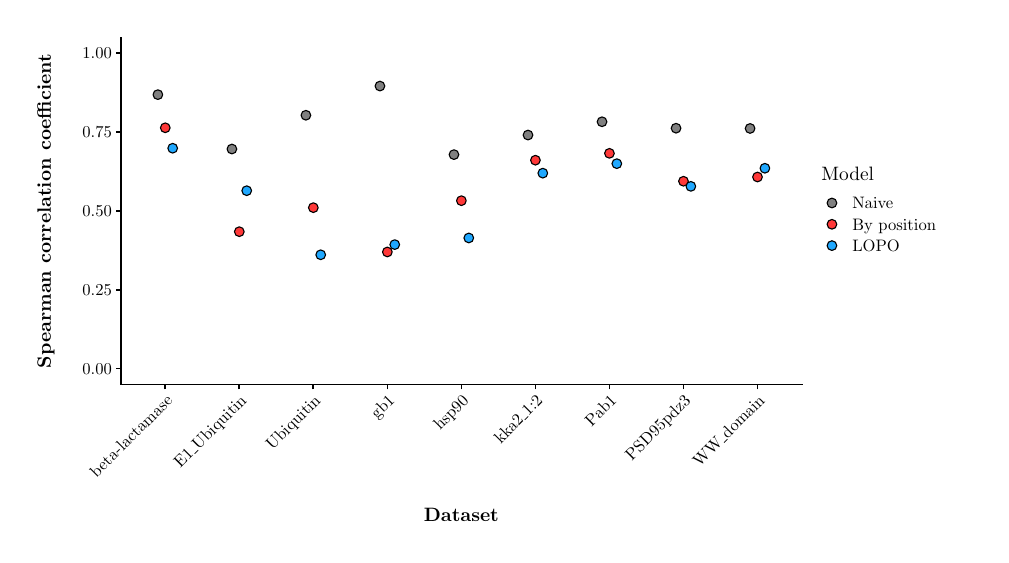
\begin{tikzpicture}[x=1pt,y=1pt]
	\definecolor{fillColor}{RGB}{255,255,255}
	\path[use as bounding box,fill=fillColor,fill opacity=0.00] (0,0) rectangle (344.26,183.39);
	\begin{scope}
		\path[clip] ( 33.67, 54.47) rectangle (279.77,179.89);
		\definecolor{drawColor}{RGB}{0,0,0}
		\definecolor{fillColor}{RGB}{128,128,128}

		\path[draw=drawColor,line width= 0.4pt,line join=round,line cap=round,fill=fillColor] ( 73.80,139.54) circle (  1.75);

		\path[draw=drawColor,line width= 0.4pt,line join=round,line cap=round,fill=fillColor] (234.29,147.06) circle (  1.75);

		\path[draw=drawColor,line width= 0.4pt,line join=round,line cap=round,fill=fillColor] (207.54,149.39) circle (  1.75);

		\path[draw=drawColor,line width= 0.4pt,line join=round,line cap=round,fill=fillColor] (100.54,151.74) circle (  1.75);

		\path[draw=drawColor,line width= 0.4pt,line join=round,line cap=round,fill=fillColor] (261.04,146.97) circle (  1.75);

		\path[draw=drawColor,line width= 0.4pt,line join=round,line cap=round,fill=fillColor] ( 47.05,159.19) circle (  1.75);

		\path[draw=drawColor,line width= 0.4pt,line join=round,line cap=round,fill=fillColor] (127.29,162.29) circle (  1.75);

		\path[draw=drawColor,line width= 0.4pt,line join=round,line cap=round,fill=fillColor] (154.04,137.52) circle (  1.75);

		\path[draw=drawColor,line width= 0.4pt,line join=round,line cap=round,fill=fillColor] (180.79,144.59) circle (  1.75);
		\definecolor{fillColor}{RGB}{255,56,56}

		\path[draw=drawColor,line width= 0.4pt,line join=round,line cap=round,fill=fillColor] ( 76.47,109.67) circle (  1.75);

		\path[draw=drawColor,line width= 0.4pt,line join=round,line cap=round,fill=fillColor] (236.97,127.90) circle (  1.75);

		\path[draw=drawColor,line width= 0.4pt,line join=round,line cap=round,fill=fillColor] (210.22,137.98) circle (  1.75);

		\path[draw=drawColor,line width= 0.4pt,line join=round,line cap=round,fill=fillColor] (103.22,118.35) circle (  1.75);

		\path[draw=drawColor,line width= 0.4pt,line join=round,line cap=round,fill=fillColor] (263.72,129.43) circle (  1.75);

		\path[draw=drawColor,line width= 0.4pt,line join=round,line cap=round,fill=fillColor] ( 49.72,147.21) circle (  1.75);

		\path[draw=drawColor,line width= 0.4pt,line join=round,line cap=round,fill=fillColor] (129.97,102.34) circle (  1.75);

		\path[draw=drawColor,line width= 0.4pt,line join=round,line cap=round,fill=fillColor] (156.72,120.87) circle (  1.75);

		\path[draw=drawColor,line width= 0.4pt,line join=round,line cap=round,fill=fillColor] (183.47,135.50) circle (  1.75);
		\definecolor{fillColor}{RGB}{31,168,255}

		\path[draw=drawColor,line width= 0.4pt,line join=round,line cap=round,fill=fillColor] (186.14,130.82) circle (  1.75);

		\path[draw=drawColor,line width= 0.4pt,line join=round,line cap=round,fill=fillColor] (159.39,107.40) circle (  1.75);

		\path[draw=drawColor,line width= 0.4pt,line join=round,line cap=round,fill=fillColor] (212.89,134.25) circle (  1.75);

		\path[draw=drawColor,line width= 0.4pt,line join=round,line cap=round,fill=fillColor] (132.64,105.00) circle (  1.75);

		\path[draw=drawColor,line width= 0.4pt,line join=round,line cap=round,fill=fillColor] (105.89,101.32) circle (  1.75);

		\path[draw=drawColor,line width= 0.4pt,line join=round,line cap=round,fill=fillColor] ( 79.15,124.48) circle (  1.75);

		\path[draw=drawColor,line width= 0.4pt,line join=round,line cap=round,fill=fillColor] (239.64,126.05) circle (  1.75);

		\path[draw=drawColor,line width= 0.4pt,line join=round,line cap=round,fill=fillColor] (266.39,132.59) circle (  1.75);

		\path[draw=drawColor,line width= 0.4pt,line join=round,line cap=round,fill=fillColor] ( 52.40,139.83) circle (  1.75);
	\end{scope}
	\begin{scope}
		\path[clip] (  0.00,  0.00) rectangle (344.26,183.39);
		\definecolor{drawColor}{RGB}{0,0,0}

		\path[draw=drawColor,line width= 0.6pt,line join=round,line cap=rect] ( 33.67, 54.47) --
		( 33.67,179.89);
	\end{scope}
	\begin{scope}
		\path[clip] (  0.00,  0.00) rectangle (344.26,183.39);
		\definecolor{drawColor}{RGB}{0,0,0}

		\node[text=drawColor,anchor=base east,inner sep=0pt, outer sep=0pt, scale=  0.60] at ( 30.42, 58.11) {0.00};

		\node[text=drawColor,anchor=base east,inner sep=0pt, outer sep=0pt, scale=  0.60] at ( 30.42, 86.61) {0.25};

		\node[text=drawColor,anchor=base east,inner sep=0pt, outer sep=0pt, scale=  0.60] at ( 30.42,115.11) {0.50};

		\node[text=drawColor,anchor=base east,inner sep=0pt, outer sep=0pt, scale=  0.60] at ( 30.42,143.62) {0.75};

		\node[text=drawColor,anchor=base east,inner sep=0pt, outer sep=0pt, scale=  0.60] at ( 30.42,172.12) {1.00};
	\end{scope}
	\begin{scope}
		\path[clip] (  0.00,  0.00) rectangle (344.26,183.39);
		\definecolor{drawColor}{RGB}{0,0,0}

		\path[draw=drawColor,line width= 0.6pt,line join=round] ( 31.92, 60.17) --
		( 33.67, 60.17);

		\path[draw=drawColor,line width= 0.6pt,line join=round] ( 31.92, 88.68) --
		( 33.67, 88.68);

		\path[draw=drawColor,line width= 0.6pt,line join=round] ( 31.92,117.18) --
		( 33.67,117.18);

		\path[draw=drawColor,line width= 0.6pt,line join=round] ( 31.92,145.68) --
		( 33.67,145.68);

		\path[draw=drawColor,line width= 0.6pt,line join=round] ( 31.92,174.19) --
		( 33.67,174.19);
	\end{scope}
	\begin{scope}
		\path[clip] (  0.00,  0.00) rectangle (344.26,183.39);
		\definecolor{drawColor}{RGB}{0,0,0}

		\path[draw=drawColor,line width= 0.6pt,line join=round,line cap=rect] ( 33.67, 54.47) --
		(279.77, 54.47);
	\end{scope}
	\begin{scope}
		\path[clip] (  0.00,  0.00) rectangle (344.26,183.39);
		\definecolor{drawColor}{RGB}{0,0,0}

		\path[draw=drawColor,line width= 0.6pt,line join=round] ( 49.72, 52.72) --
		( 49.72, 54.47);

		\path[draw=drawColor,line width= 0.6pt,line join=round] ( 76.47, 52.72) --
		( 76.47, 54.47);

		\path[draw=drawColor,line width= 0.6pt,line join=round] (103.22, 52.72) --
		(103.22, 54.47);

		\path[draw=drawColor,line width= 0.6pt,line join=round] (129.97, 52.72) --
		(129.97, 54.47);

		\path[draw=drawColor,line width= 0.6pt,line join=round] (156.72, 52.72) --
		(156.72, 54.47);

		\path[draw=drawColor,line width= 0.6pt,line join=round] (183.47, 52.72) --
		(183.47, 54.47);

		\path[draw=drawColor,line width= 0.6pt,line join=round] (210.22, 52.72) --
		(210.22, 54.47);

		\path[draw=drawColor,line width= 0.6pt,line join=round] (236.97, 52.72) --
		(236.97, 54.47);

		\path[draw=drawColor,line width= 0.6pt,line join=round] (263.72, 52.72) --
		(263.72, 54.47);
	\end{scope}
	\begin{scope}
		\path[clip] (  0.00,  0.00) rectangle (344.26,183.39);
		\definecolor{drawColor}{RGB}{0,0,0}

		\node[text=drawColor,rotate= 45.00,anchor=base east,inner sep=0pt, outer sep=0pt, scale=  0.60] at ( 52.64, 48.30) {beta-lactamase};

		\node[text=drawColor,rotate= 45.00,anchor=base east,inner sep=0pt, outer sep=0pt, scale=  0.60] at ( 79.39, 48.30) {E1\_Ubiquitin};

		\node[text=drawColor,rotate= 45.00,anchor=base east,inner sep=0pt, outer sep=0pt, scale=  0.60] at (106.14, 48.30) {Ubiquitin};

		\node[text=drawColor,rotate= 45.00,anchor=base east,inner sep=0pt, outer sep=0pt, scale=  0.60] at (132.89, 48.30) {gb1};

		\node[text=drawColor,rotate= 45.00,anchor=base east,inner sep=0pt, outer sep=0pt, scale=  0.60] at (159.64, 48.30) {hsp90};

		\node[text=drawColor,rotate= 45.00,anchor=base east,inner sep=0pt, outer sep=0pt, scale=  0.60] at (186.39, 48.30) {kka2\_1:2};

		\node[text=drawColor,rotate= 45.00,anchor=base east,inner sep=0pt, outer sep=0pt, scale=  0.60] at (213.14, 48.30) {Pab1};

		\node[text=drawColor,rotate= 45.00,anchor=base east,inner sep=0pt, outer sep=0pt, scale=  0.60] at (239.89, 48.30) {PSD95pdz3};

		\node[text=drawColor,rotate= 45.00,anchor=base east,inner sep=0pt, outer sep=0pt, scale=  0.60] at (266.64, 48.30) {WW\_domain};
	\end{scope}
	\begin{scope}
		\path[clip] (  0.00,  0.00) rectangle (344.26,183.39);
		\definecolor{drawColor}{RGB}{0,0,0}

		\node[text=drawColor,anchor=base,inner sep=0pt, outer sep=0pt, scale=  0.70] at (156.72,  4.86) {\bfseries Dataset};
	\end{scope}
	\begin{scope}
		\path[clip] (  0.00,  0.00) rectangle (344.26,183.39);
		\definecolor{drawColor}{RGB}{0,0,0}

		\node[text=drawColor,rotate= 90.00,anchor=base,inner sep=0pt, outer sep=0pt, scale=  0.70] at (  8.39,117.18) {\bfseries Spearman correlation coefficient};
	\end{scope}
	\begin{scope}
		\path[clip] (  0.00,  0.00) rectangle (344.26,183.39);
		\definecolor{drawColor}{RGB}{0,0,0}

		\node[text=drawColor,anchor=base west,inner sep=0pt, outer sep=0pt, scale=  0.70] at (286.77,128.07) {Model};
	\end{scope}
	\begin{scope}
		\path[clip] (  0.00,  0.00) rectangle (344.26,183.39);
		\definecolor{drawColor}{RGB}{0,0,0}
		\definecolor{fillColor}{RGB}{128,128,128}

		\path[draw=drawColor,line width= 0.4pt,line join=round,line cap=round,fill=fillColor] (290.62,120.04) circle (  1.75);
	\end{scope}
	\begin{scope}
		\path[clip] (  0.00,  0.00) rectangle (344.26,183.39);
		\definecolor{drawColor}{RGB}{0,0,0}
		\definecolor{fillColor}{RGB}{255,56,56}

		\path[draw=drawColor,line width= 0.4pt,line join=round,line cap=round,fill=fillColor] (290.62,112.34) circle (  1.75);
	\end{scope}
	\begin{scope}
		\path[clip] (  0.00,  0.00) rectangle (344.26,183.39);
		\definecolor{drawColor}{RGB}{0,0,0}
		\definecolor{fillColor}{RGB}{31,168,255}

		\path[draw=drawColor,line width= 0.4pt,line join=round,line cap=round,fill=fillColor] (290.62,104.64) circle (  1.75);
	\end{scope}
	\begin{scope}
		\path[clip] (  0.00,  0.00) rectangle (344.26,183.39);
		\definecolor{drawColor}{RGB}{0,0,0}

		\node[text=drawColor,anchor=base west,inner sep=0pt, outer sep=0pt, scale=  0.60] at (297.97,117.97) {Naive};
	\end{scope}
	\begin{scope}
		\path[clip] (  0.00,  0.00) rectangle (344.26,183.39);
		\definecolor{drawColor}{RGB}{0,0,0}

		\node[text=drawColor,anchor=base west,inner sep=0pt, outer sep=0pt, scale=  0.60] at (297.97,110.27) {By position};
	\end{scope}
	\begin{scope}
		\path[clip] (  0.00,  0.00) rectangle (344.26,183.39);
		\definecolor{drawColor}{RGB}{0,0,0}

		\node[text=drawColor,anchor=base west,inner sep=0pt, outer sep=0pt, scale=  0.60] at (297.97,102.57) {LOPO};
	\end{scope}
\end{tikzpicture}
